To solve the constrained optimization problem \eqref{eq:disoTPS_YB_move_alternative_formulation} we proceed by maximizing the overlap while only varying the parameters of one of the three tensors $T^\prime$, $W_1^\prime$ or $W_2^\prime$, treating all other tensors as constant. For example, let us keep $W_1^\prime$ and $W_2^\prime$ fixed and optimize $T^\prime$. We first contract all tensors except $T^\prime$ into an environment $E$ as shown in figure \figref{fig:YB_move_iterate_polar_optimize_T}. We can then write the optimization problem as
\begin{equation}
	T^\prime_\text{opt} = \underset{T^{\prime\dagger}T = \id}{\argmax} \Re\left\langle\Psi\middle|\Psi^\prime\right\rangle = \underset{T^{\prime\dagger}T = \id}{\argmax}\Re\left\langle E, T^\prime\right\rangle_\text{F} = \underset{T^{\prime\dagger}T = \id}{\argmax}\Re\Tr\left(T^{\prime\dagger}E\right).
\end{equation}
This problem is known as the \textit{orthogonal Procrustes problem} and permits the closed form solution $T^\prime_\text{opt} = UV^\dagger$, where $U$ and $V$ are computed using the SVD $E = USV^\dagger$. For the derivation of this solution see appendix \ref{app:optimization_problems_for_isometric_tensor_networks}. The tensors $W_1^\prime$ and $W_2^\prime$ can be optimized similarly. The full algorithm is then performed by sweeping over the three tensors, optimizing them iteratively until convergence. Tensor diagrams for the algorithm are shown in figure \figref{fig:YB_move_iterate_polar}. We discuss one iteration of the algorithm in more detail:
\begin{enumerate}
	\item Contract all tensors except $T^\prime$ into an environment $E$ and perform an SVD $E = USV$. The tensor $T^\prime$ is then updated as $T^\prime\leftarrow UV^\dagger$. See figure \figref{fig:YB_move_iterate_polar_optimize_T}.
	\item Contract all tensors except $W_1^\prime$ into an environment $E$ and perform an SVD $E = USV$. The tensor $W_1^\prime$ is then updated as $W_1^\prime\leftarrow UV^\dagger$. See figure \figref{fig:YB_move_iterate_polar_optimize_W1}.
	\item Contract all tensors except $W_2^\prime$ into an environment $E$. The tensor $W_1^\prime$ is then updated as $W_1^\prime\leftarrow E/\left\lVert E\right\rVert$. See figure \figref{fig:YB_move_iterate_polar_optimize_W2}.
\end{enumerate}
These three steps are repeated until a termination criterion is met, for example until the decrease in error after one iteration is smaller than a given threshold or if a given maximum number of iterations $N_\text{iter}$ is exceeded. A similar algorithm was also used by Evenbly and Vidal in the context of the multi-scale entanglement renormalization ansatz
(MERA) \cite{cite:algorithms_for_entanglement_renormalization, cite:algorithms_for_entanglement_renormalization_boundaries_impurities_interfaces}. Note that in step three of the algorithm, a norm constraint is enforced instead of an isometry constraint, in which case the closed form solution takes a different shape. We also derive this solution in appendix \ref{app:optimization_problems_for_isometric_tensor_networks}.\par
\begin{figure}
	\centering
	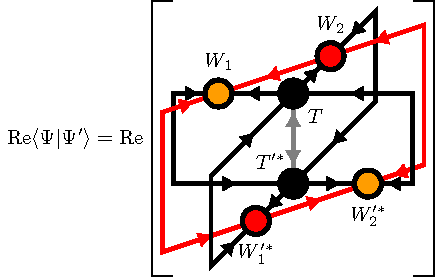
\includegraphics[scale=1]{figures/tikz/disoTPS/yang_baxter_move_iterative/yang_baxter_move_iterative_a.pdf}
	\caption{The cost function of the optimization problem \eqref{eq:disoTPS_YB_move_alternative_formulation} can be computed as a contraction of only six tensors.}
	\label{fig:YB_move_iterate_polar_overlap}
\end{figure}
\begin{figure}
	\centering
	\begin{subfigure}[c]{0.85\textwidth}
		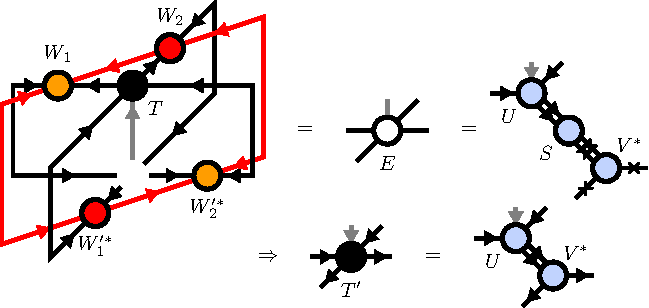
\includegraphics[scale=1]{figures/tikz/disoTPS/yang_baxter_move_iterative/yang_baxter_move_iterative_b.pdf}
		\caption{}\label{fig:YB_move_iterate_polar_optimize_T}
	\end{subfigure}
	\begin{subfigure}[c]{0.85\textwidth}
		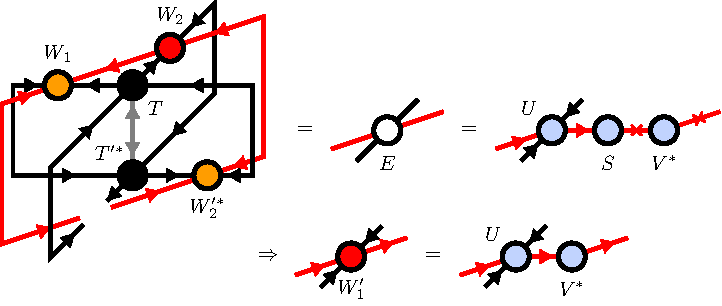
\includegraphics[scale=1]{figures/tikz/disoTPS/yang_baxter_move_iterative/yang_baxter_move_iterative_c.pdf}
		\caption{}\label{fig:YB_move_iterate_polar_optimize_W1}
	\end{subfigure}
	\begin{subfigure}[c]{0.85\textwidth}
		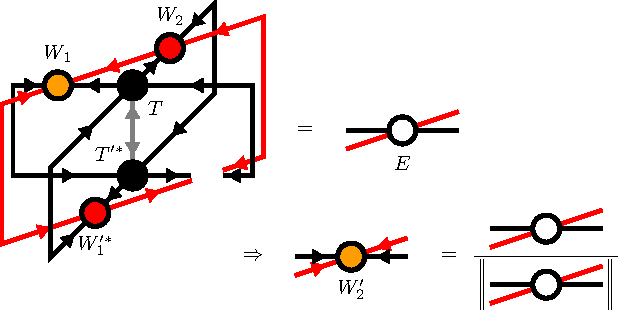
\includegraphics[scale=1]{figures/tikz/disoTPS/yang_baxter_move_iterative/yang_baxter_move_iterative_d.pdf}
		\caption{}\label{fig:YB_move_iterate_polar_optimize_W2}
	\end{subfigure}%
	\caption{In this figure we show the three local updates that are used to iteratively solve optimization problem \eqref{eq:disoTPS_YB_move_alternative_formulation}. (a) The tensor $T^\prime$ can be updated similarly by contracting all tensors except $T^\prime$ into the environment $E$ and isometrizing $E$ using an SVD. (b) The tensor $W_1^\prime$ can be updated by contracting all tensors except $W_1^\prime$ into the environment $E$, which is subsequently isometrized using an SVD. (c) To optimize the tensor $W_2^\prime$, all tensors except $W_2^\prime$ are contracted into the environment $E$. The updated tensor is then given as $W_2^\prime = E/\lVert E\rVert$.}
	\label{fig:YB_move_iterate_polar}
\end{figure}
The computational cost of the algorithm is dominated by the tensor contractions, scaling as $\mathcal{O}(3N_\text{iter}(\chi^2D^6d + \chi^3D^4)) = \mathcal{O}(N_\text{iter}D^8)$ for one YB move.\par
\begin{figure}
	\centering
	\begin{tikzpicture}[scale=1, trim axis left, trim axis right]
		\begin{axis}[xlabel=$N_\text{iters}$, ylabel={$\lVert|\Psi\rangle-|\Psi^\prime\rangle\rVert$}, grid=both, grid style={gray!20}, every axis plot/.append style={very thick}, scale only axis, height=\singleFigureHeight, width=\singleFigureWidth]
			
			\addplot[color = 5blue4]
			table[x=N_iter, y=trunc_error, col sep=space]{figures/plots/disoTPS/data/iterate_polar.txt};
			%\addlegendentry{Evenbly-Vidal}
			
		\end{axis}
	\end{tikzpicture}
	\caption{We show a cool figure here!!\todo{Caption}}
	\label{fig:disoTPS_tripartite_decomposition_iterate_polar}
\end{figure}
In practice we observe that the discussed algorithm converges only very slowly. To qualitatively showcase this, we perform the YB move on a typical environment of tensors $\left\{W_1, W_2, T\right\}$ that was encountered during imaginary time evolution of the Transverse Field Ising model, see chapter \ref{chap:TFI} for more details. The bond dimensions chosen for the disoTPS are $D = 4$, $\chi = 24$. \par. We plot the error $\lVert|\Psi\rangle-|\Psi^\prime\rangle\rVert$ against the number of iterations in figure \figref{fig:disoTPS_tripartite_decomposition_iterate_polar}. After $N_\text{iter}=10000$ iterations, the algorithm is still not converged.